\chapter{Chapitre 1}

\section{Le couplage en transport : du direct à l'indirect}

Lorsque l'on souhaite sonder le magnétisme moléculaire par une mesure en courant, il faut que le "chemin" emprunté par les électrons soit très proche du centre magnétique. On peut, dans ce cadre, imaginer deux configurations : le couplage direct, où les électrons impliqués dans le transport jouent également un rôle direct dans le magnétisme de la molécule sondée; le couplage indirect, dans lequel les électrons impliqués dans le courant ne contribuent pas au magnétisme de la molécule, mais le perturbent légèrement. Suivant la configuration adoptée, le mode de mesures sera différent, tout comme le sera l'impact sur le magnétisme. C'est ce que nous allons détailler maintenant.

\subsection{Le couplage direct}
Le couplage direct implique que les électrons responsable du courant jouent également un rôle dans le magnétisme de la molécule. Cette dernière va osciller entre deux états de charge N/N+1 , chacun d'eux ayant sa propre configuration magnétique. L'analyse se fait en sondant la différence en énergie des différentes transitions N/N+1, le plus souvent par une technique de spectroscopie en tunnelling séquentiel~(cf chapitre théorique). Le principal avantage de cette technique est qu'elle permet d'étudier différents états de charge~(nombre d'oxydation ou de réduction). En revanche, le caractère très invasif de la méthode ne permet pas d'espérer de long temps de vie pour les différents états du système. Cette méthode a été mise en œuvre expérimentalement dans [mettre les citations] avec des résultats mitigés, du fait notamment de la dégradation de la molécule lors de la fabrication du dispositif. Des études théoriques ont également été menées, permettant une analyse plus fine des résultats expérimentaux.

\subsection{Le couplage indirect}

Dans le cas du couplage indirect, les électrons responsables du courant ne participent qu'indirectement au magnétisme de la molécule. La mesure se fait par l'analyse statistique des modifications de conductance du système en fonction du champ magnétique, la polarisation en tension source-drain et grille étant en général fixée~(par opposition à la spectroscopie en tunneling séquentiel). Dans cette configuration, le nombre d'électron impliqués dans le magnétisme moléculaire ne peut pas être modifié. En revanche, la technique de mesure par couplage indirect se révèle beaucoup moins invasive. Cela garantie d'une part, la préservation des propriétés magnétique et d'autre part, l'observation de long temps de vie. Cette configuration a été utilisé dans deux dispositifs légèrement différents. Dans le premier, une deuxième molécule~(un nanotube) a été utilisée comme point quantique sonde, l'aimant moléculaire étant déposé sur sa surface [citation de Matias]. Dans le deuxième dispositif, le cœur magnétique étant fortement découplé des ligands périphériques, ces derniers ont joué le rôle de point quantique sonde[nous]. Quelques outils théoriques sont venus faciliter l'interprétation des résultats [papier sur nanotube] mais également proposer de nouvelles expériences [article du les ligand et couple mécanique].

\section{Le couplage magnétique}
Dans la configuration directe présenté précédemment, le couplage entre le courant et le magnétisme est aisé à comprendre, les électrons participant au premier étant également directement impliqués dans le second. En revanche, dans la configuration indirecte, le couplage entre ces deux domaines peut avoir plusieurs origines. Il a pour conséquence de rendre le potentiel chimique du point quantique dépendant du centre magnétique. Cette dépendance est fonction de la nature de l'interaction comme nous allons le montrer maintenant.

\subsection{Origine dipolaire}
Le couplage dipolaire est une interaction à distance entre deux moments magnétiques. Chacun de ces moments génère un champ dipolaire qui va venir agir sur le second, et vice versa. La modification en énergie induite est fonction de la distance séparant les deux dipôles, ainsi que de leur orientation relative. Ceci s'exprime par:
\begin{eqnarray}
E = -\frac{\mu_0 \mu_B}{4\pi r^3}(3\mathbf{SnJn} - \mathbf{SJ}) \nonumber
\end{eqnarray}

\begin{figure}
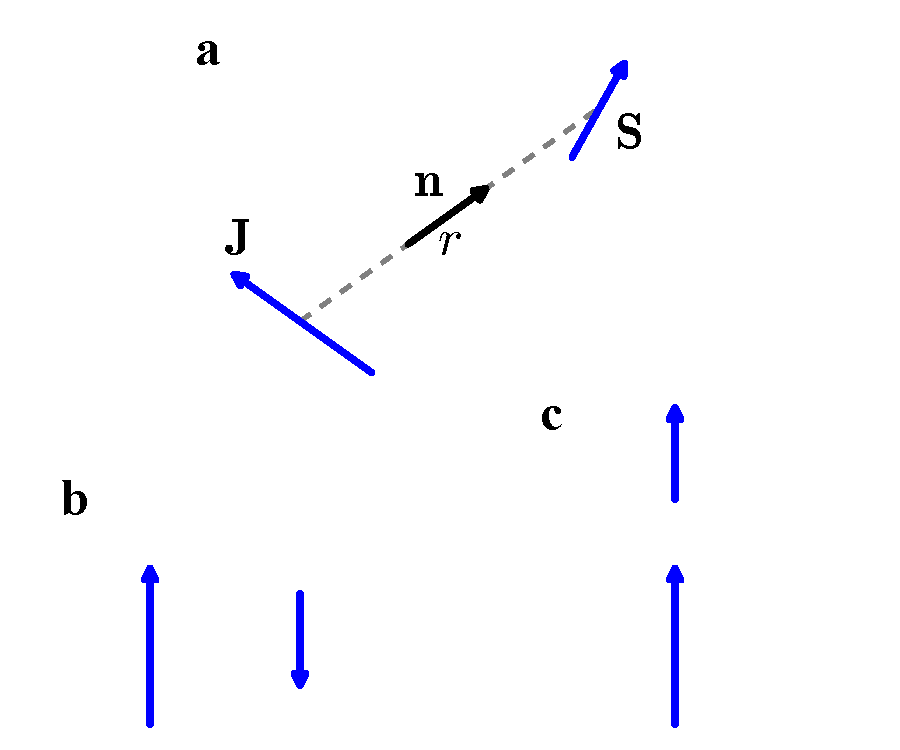
\includegraphics[scale=0.5]{Resultats/Chap1/Figure1/figure1.pdf} 
\caption{}
\label{dipolaire}
\end{figure}

où $\mathbf{S}$ et $\mathbf{J}$ sont les spins associés au deux moment magnétiques, $r$ la distance qui les sépare et $\mathbf{n}$ la normale reliant les deux moments (cf figure??). Plusieurs remarques s'imposent. Premièrement, l'intensité de l'interaction est proportionnelle à l'inverse de la distance au cube. Elle devient très rapidement négligeable : pour un spin $J=6$, elle ne vaut plus que $10$\,mT à $1$\,nm. Deuxièmement, on peut imaginer deux configurations opposées : dans la situation de la figure??, le couplage abouti à une organisation anti-ferromagnétique; dans celle présentée dans la figure ??, le couplage est au contraire ferromagnétique. Dans le cas de TbPc$_2$, le plan des ligands est perpendiculaire à l'axe facile du moment magnétique ce qui correspond plutôt à la seconde configuration. De plus, la seule transition possible à basse température est $J_z=\pm6 \rightarrow J_z \mp 6$. Si l'on tient compte de ces remarques, la variation du potentiel chimique du point quantique sonde $\mu_{QD}$ est liée au renversement du moment magnétique par :
\begin{eqnarray}
\Delta \mu_{QD} = -\frac{\mu_0 \mu_B}{2\pi r^3}S_z\Delta J_z\nonumber
\end{eqnarray}
Celle-ci est directement proportionnelle à $\Delta J_z$.

\subsection{Couplage d'échange}
Le couplage d'échange est une interaction de contact entre deux moments magnétiques. Elle résulte d'un recouvrement des fonctions d'onde et peut favoriser deux situations opposés : si elle est de type ferromagnétique, les spins s'alignent entre deux ; si elle est de type anti-ferromagnétique, l'orientation entre spin est opposée. Cette interaction s'exprime comme suit :
\begin{eqnarray}
E = A\mathbf{SJ} \nonumber
\end{eqnarray}
où $A$ est la constante d'échange. Lorsque $A>0$, le couplage est anti-ferromagnétique, si $A<0$, il est ferromagnétique. La constante d'échange peut prendre des valeurs élevées en énergie : dans le cas du N@C$_{60}$ par exemple, la valeur de l'échange entre le spin de l'azote et les électrons du C$_{60}$ a été mesurée supérieure à 4\,T. Si l'on tient compte des considérations évoquées dans le cas du couplage dipolaire, la modification d\^u à l'interaction d'échange qu’entraîne un retournement de l'aimantation peut s'exprimer de la façon suivante :
\begin{eqnarray}
\Delta \mu_{QD} = AS_z\Delta J_z\nonumber
\end{eqnarray}
Cette expression est semblable à celle obtenue pour le couplage dipolaire. Dans le cas où $A<0$ , les deux interactions produisent même des effets identiques. La principale différence réside dans l'intensité de l'interaction : si celle-ci est de l'ordre du mT, elle est certainement dipolaire; si elle est en revanche de l'ordre de quelques dizaines de mT, l'interaction d'échange est l'interaction dominante.

\subsection{Le couplage magnéto-Coulomb}
L'origine de ce couplage est électrostatique. Si l'on considère un point quantique et un centre magnétique, cette interaction va coupler le potentiel chimique du premier à celui du second de telle sorte que :
\begin{eqnarray}
\Delta \mu_{QD} = C_{mc} \Delta \mu_{CM}
\end{eqnarray}
où $C_{mc}$ est la constate de couplage et $\Delta \mu_{CM}$ la variation du potentiel chimique du centre magnétique. Cette expression peut être simplifiée, au regard des remarques précédentes, de la façon suivante :
\begin{eqnarray}
\Delta \mu_{QD} = C_{mc} g \mu_B  \Delta J_z B_z
\end{eqnarray}
Contrairement aux expressions précédentes, la variations du potentiel chimique associée à un retournement de l'aimantation n'est pas constante mais dépend du champ magnétique appliqué. Cela rend cette dernière facile à identifier.

\section{Nature et intensité de l'interaction}
L'analyse de nos résultats passe par l'identification de l'interaction mise en jeu dans notre méthode de détection. Deux paramètres sont à évaluer pour clairement en identifier la nature : la dépendance en champ magnétique de la variation du potentiel chimique et l'intensité de l'interaction. Nous allons nous attacher à quantifier ces deux paramètres à l'aide de mesure en transport. La première étape sera consacré à l'étude de la hauteur des sauts de conductance. La seconde s'appuiera sur une étude de l'effet Kondo et sur l'influence de l'interaction sur ce dernier.

\subsection{Amplitude du saut de conductance}
Dans le chapitre théorique, nous avons montré que le potentiel chimique du point quantique était directement relié à la conductance différentielle mesurée. On peut résumer cette tendance par la relation suivante:
\begin{eqnarray}
\text{d}G = \frac{\partial G}{\partial \mu} \text{d} \mu
\end{eqnarray}
Si l'on se place dans une situation où $\frac{\partial G}{\partial \mu} = cst$, alors la variation observée en conductance sera une mesure directe de la variation du potentiel chimique. Si maintenant, on considère la variation du potentiel chimique en fonction du champ magnétique, sans renversement magnétique, on a $\text{d}\mu \propto \text{d}B$. Pour avoir $\frac{\partial G}{\partial \mu} = cst$, cela revient à se placer dans une zone ou $\frac{\partial G}{\partial B} = cst$. La Fig.??? montre une mesure de $G$ en fonction du champ magnétique $B$ et met en évidence la zone correspondante à $\frac{\partial G}{\partial B} = cst$. Dans celle-ci, un saut en conductance est directement proportionnel à la variation en potentiel chimique. Si cette dernière est dépendante en champ magnétique, la hauteur des sauts en conductance devrait également l’être. Or, la mesure présentée dans Fig.?? montre clairement que la hauteur des sauts en conductance, et donc la variation du potentiel chimique, ne dépend pas du champ magnétique. Cette première observation nous permet d'éliminer l'interaction de type magnéto-Coulomb des mécanismes de coulage possible. On a donc à faire, soit à un couplage dipolaire, soit à un couplage d'échange. Seule l'analyse de l'intensité de l'interaction peut nous renseigner et c'est à sa détermination que nous allons nous attacher maintenant.

\begin{figure}
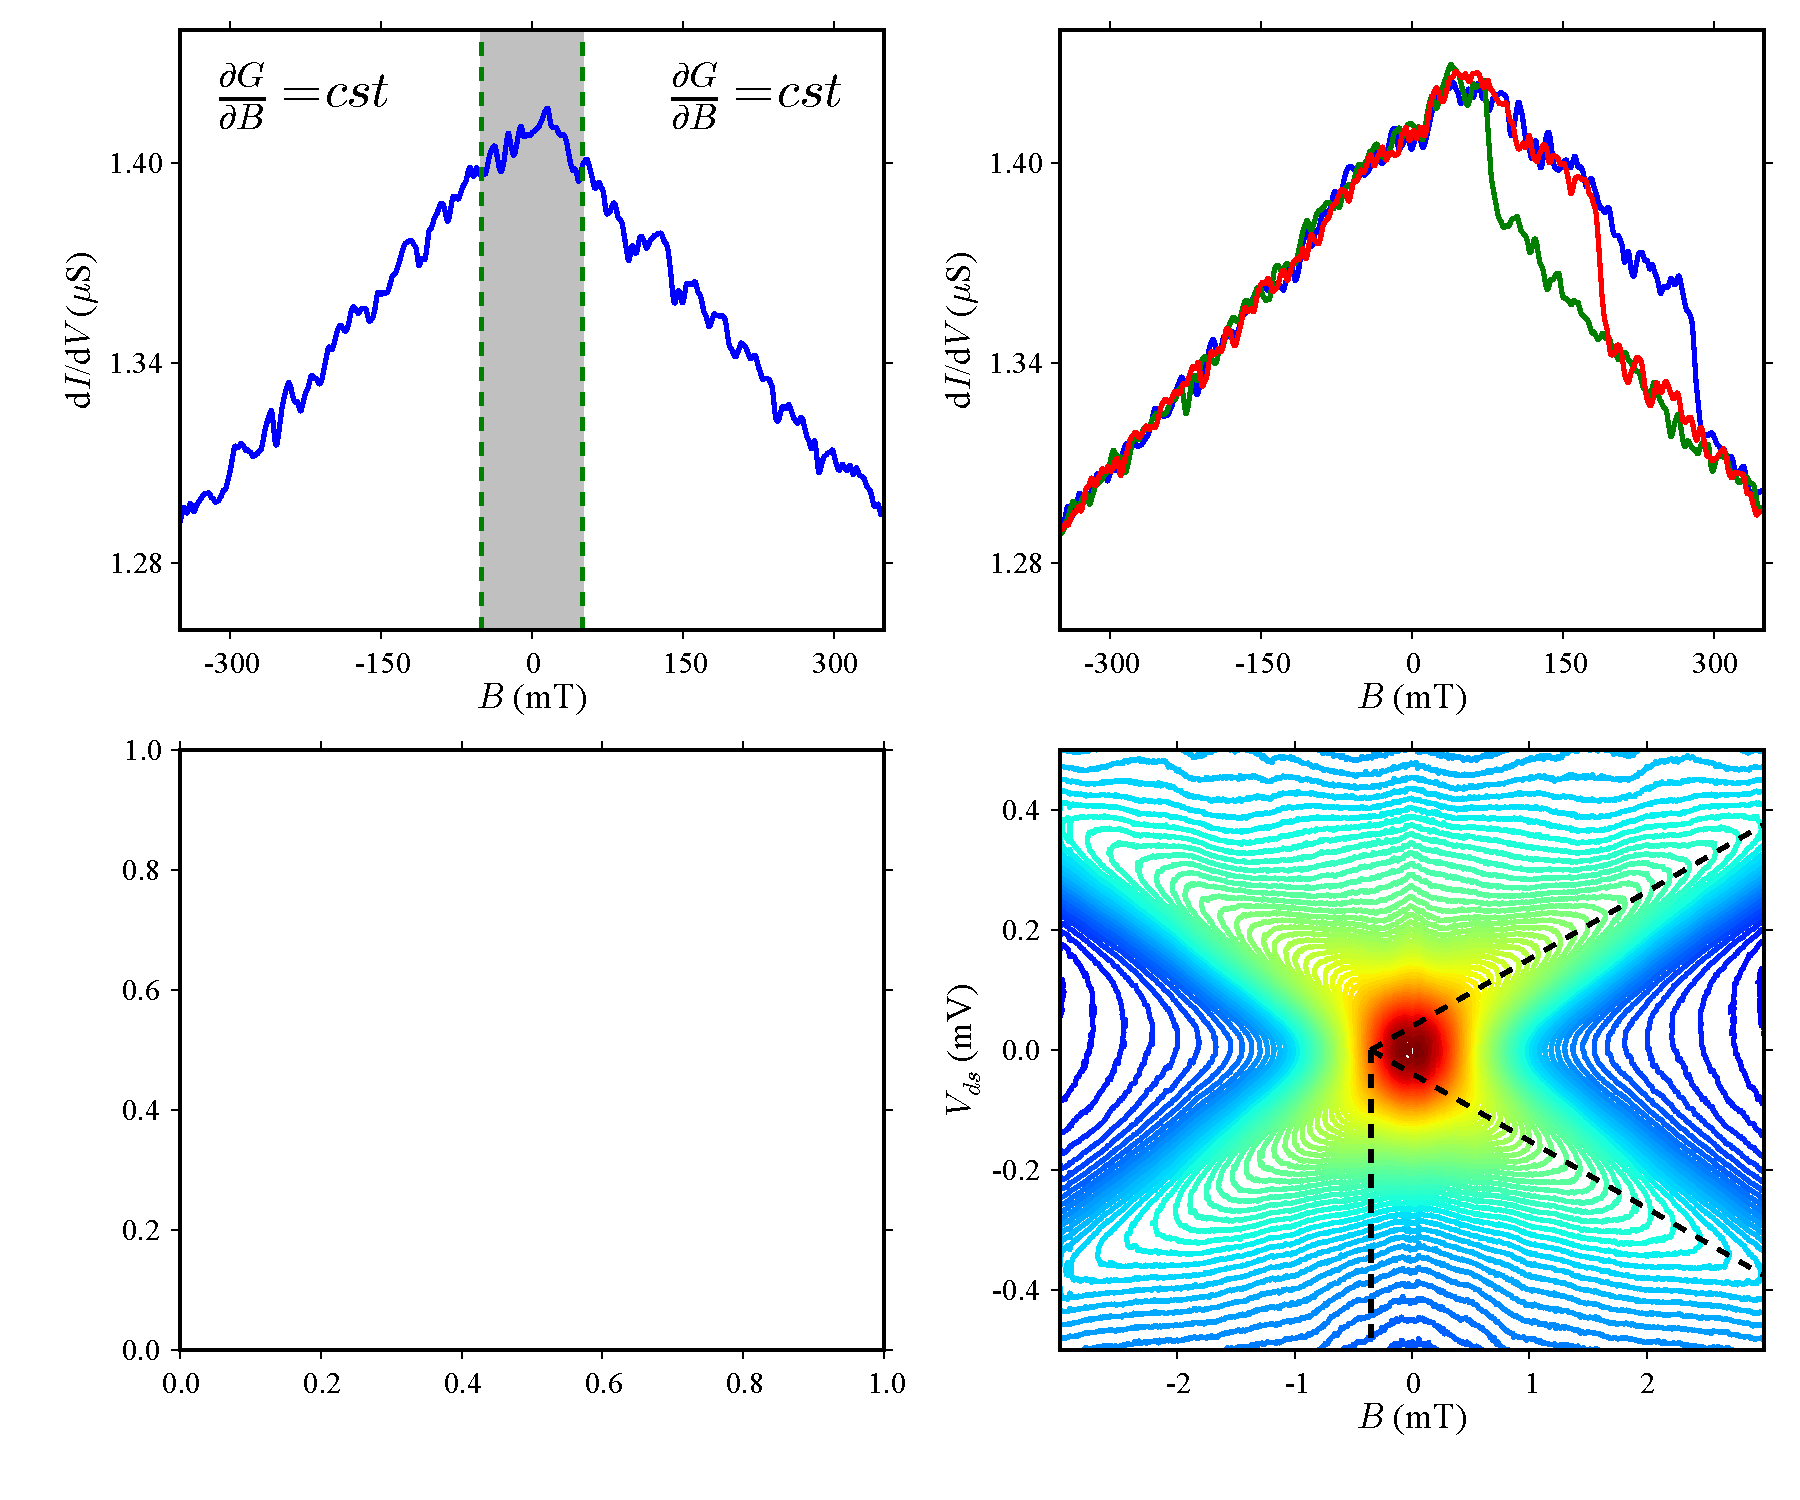
\includegraphics[scale=0.5]{Resultats/Chap1/Figure2/figure2.pdf} 
\caption{}
\label{analyse_interaction}
\end{figure}

\subsection{Intensité de l'interaction}
L'intensité de l'interaction peut s'obtenir en comparant un système découplé de l'interaction avec le même système la subissant. Pour cela, on peut s'appuyer sur un phénomène universel tel l'effet Kondo de spin 1/2.

\subsubsection{L'effet Kondo 1/2}
La Fig??? présente la mesure d'un effet Kondo 1/2 en fonction du champ magnétique et de la tension source drain. \`A $B=0$, on observe un pic de conductance à tension source-drain nulle. Lorsque l'on applique un champ magnétique, ce pic s'étale puis, puis se divise en deux pics de conductance. Cette séparation est directement induite par l'effet Zeeman. En extrapolant les maxima pour différentes valeurs du champ magnétique, on obtient une lecture de l'écartement Zeeman. En revanche, contrairement à ce que l'on pourrait attendre, les droites ne se croisent pas en $B=0$, mais en une valeur de champ fini $B_c$ supérieure à zéro. La valeur de $B_c$ est directement reliée à la température Kondo $T_K$ par $k_bT_K = \mu_B B_c$. Autrement dit, il est nécessaire de fournir une énergie supérieure à celle de la température Kondo pour "casser" le singlet formé par le nuage Kondo et l'électron du point quantique. Regardons maintenant ce qu'il en est de notre système couplé.

\subsubsection{Effet Kondo du système couplé}
Si l'on effectue cette étude dans le cas du Kondo 1/2 couplé, on observe le même comportement général. Les pentes des droites extraites des extrema confirme qu'il s'agit d'un Kondo de spin 1/2. En revanche, la valeur de $B_c$ n'est plus positive mais négative. Tout se passe comme si le singlet était déjà "cassé" à champ magnétique nul. Cette première observation nous permet d'éliminer l'interaction d'échange anti-ferromagnétique. En effet, cette dernière aurait pour conséquences de décalé $B_c$ vers des valeur plus élevées de champ magnétique. On a donc à faire, soit à une interaction dipolaire, soit à une interaction d'échange ferromagnétique.

Si on néglige le décalage vers les valeurs de champ positives du champ critique $B_c$ induit par l'effet Kondo, une estimation basse de l'intensité de l'interaction peut être donné par le décalage négatif du champ critique. En effet, celui-ci étant uniquement du au couplage d'échange, l'interaction est de l'ordre de plusieurs dizaines de milliKelvin. Au regard des dimensions du système qui place le ligand à environs 1\,nm du centre magnétique, et s'agissant d'une valeur minimale, l'interaction dominante est l'interaction d'échange ferromagnétique.

\section{Analyse des sauts en conductance}
L'analyse des sauts de conductance est à la base de notre méthode de détection. C'est de leur analyse que nous allons extraire les propriétés magnétiques de notre système. Il faut pouvoir les détecter de manière efficace et pertinente en fonction de critères bien établis. Le grand nombre de mesures à traiter impose l'usage des méthodes numériques. Celle-ci doit pouvoir extraire les paramètres essentiels des sauts de conductance : leurs positions en champ magnétique, leur amplitudes et leur signes. De plus, le point de fonctionnement, c'est à dire les tensions source-drain et grille appliquées, doit être optimal afin de faciliter cette détection. Nous allons dans ce paragraphe décrire la méthode de détection des sauts. Ceci nous permettra, en particulier, de valider le lien entre variation de conductance et retournement de l'aimantation. Enfin, nous nous attarderons sur les critères de sélection du point de fonctionnement.

\begin{figure}
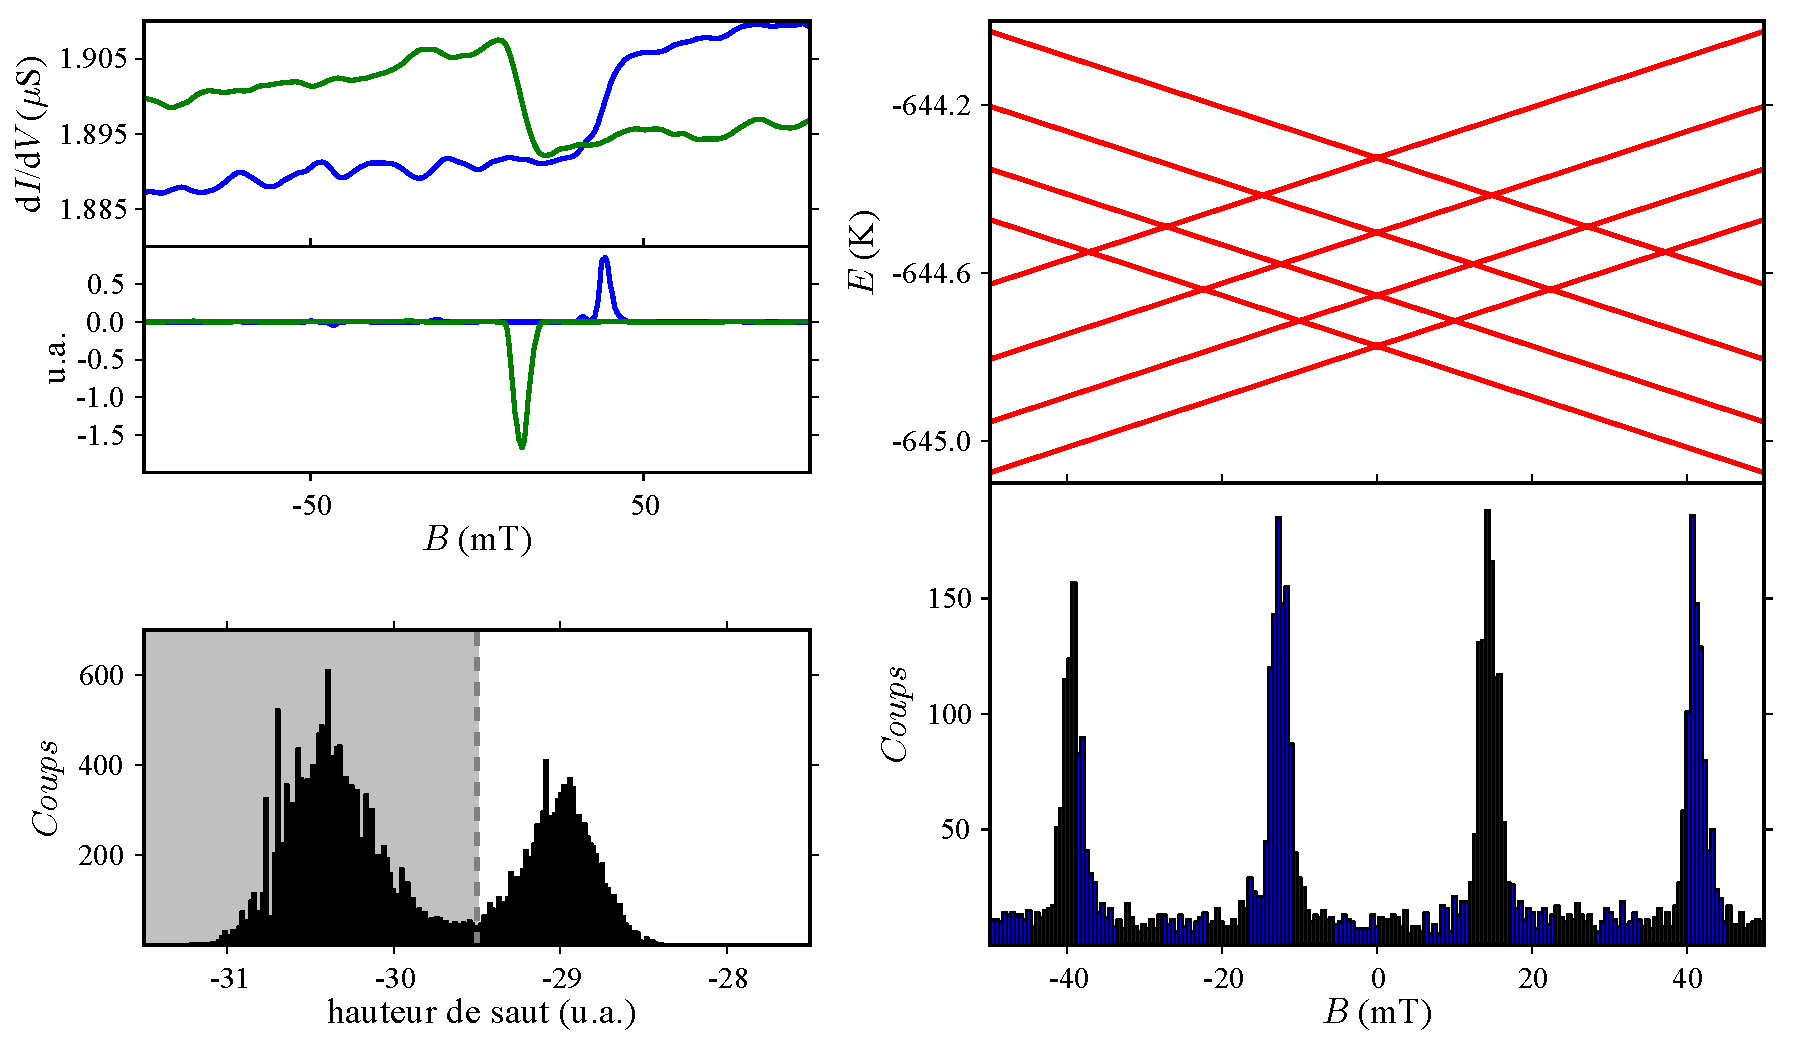
\includegraphics[scale=0.5]{Resultats/Chap1/Figure3/figure3.pdf} 
\caption{}
\label{analyse_saut}
\end{figure}

\subsection{Méthode de détection}
La première étape de notre méthode de mesure est de détecter chaque saut en conductance relative à un retournement de l'aimantation. Une mesure type d'un saut de conductance est présenté dans la Fig.???. Il faut, dans un premier temps, rendre le signal plus facilement exploitable par l'application d'un filtre détaillé dans la Fig.??. La Fig?? correspond au signal de la Fig?? après son application. Les sauts de conductances ont été converti en pic qu'il est facile d'extraire par une méthode des extrema. Le signe du saut de conductance est donné par l'orientation des pics : un changement positif correspond à un maximum; un changement négatif à un minimum.

Il faut ensuite procéder à l'analyse statistique de ces sauts. Pour cela, il faut garder à l'esprit qu'il peut y avoir des mesures sans saut, le retournement étant un événement probabiliste. Dans ce cas, les extrema détecté ne correspondront pas à un signal véritable mais à un artefact. Afin d'aboutir à un résultat convenable, il faut procéder en trois étapes. On filtre tout d'abord le signal pour extraire les différents extrema. Ensuite, pour ne prendre en compte que le signal et éliminer les artefacts, on effectue une statistique de la hauteur des pics du signal filtré. La Fig.?? présente le résultat d'une telle statistique pour ??? mesures. Deux distribution sont clairement identifiable : une distribution avec de faibles sauts correspondant au bruit de mesures; une distribution de sauts marqués correspondant à des retournement de l'aimantation. La dernière étape consistera à filtrer le signal à l'aide d'un seuil fournis par la distribution des retournement de l'aimantation.

A partir des sauts sélectionnés, on effectue une étude statistique des champs de retournement de l'aimantation. La Fig?? présente un telle statistique effectué sur ??? mesures faites à faible champ. On peut facilement identifier quatre résonances, c'est à dire, quatre valeur du champ pour lesquel l'aimantation de la molécule à une forte probabilité de se retourner. En comparant cette mesure avec le diagramme Zeeman de la molécule de TbPc2, on peut associer chaque résonance à chacun des anti-croisements repérés par des cercles. Sachant que chacun de ces croisement correspond à une situation au le QTM est possible, on peut en déduire que la présence de résonance est la mesure \textbf{directe} de la mesure de QTM à l'échelle d'une seule molécule. De plus, chaque anti-croisement est associé à un unique état de spin nucléaire. La mesure de la position en champ magnétique du retournement de l'aimantation est donc une mesure \textbf{indirecte} de l'état de spin du noyau de terbium. C'est cette dernière propriété que nous utiliserons dans la suite pour étudier la dynamique du spin nucléaire.


\subsection{Interprétation physique du signe de $\Delta$G}
Jusqu'à présent, nous n'avons pas utiliser le signe de $\Delta G$ comme élément d'analyse. Pourtant, dans le cadre de notre modèle, celui-ci donne accès à la nature de la transition : $J_z = \pm6 \rightarrow J_z = \mp 6$. Il existe une méthode expérimentale, basée sur la population thermique des spins nucléaires, permettant de vérifier notre hypothèse.

Supposons que l'on se place dans l'état initial $J_z=+6$ et $B<0$. Au regard du digramme Zeeman de la Fig?? et du fait de la relaxation, l'état de spin $I_z = -3/2$ devrait être le plus probablement mesuré, $I_z = +3/2$ étant le moins probable. L'inverse est vrai pour l'état initial $J_z=-6$ et $B<0$. La Fig??? présente une étude statistique des champs de retournement pour les cas où $\Delta G> 0$ et $\Delta G< 0$. Les 4 barres superposés à l'histogramme correspondent à l'intégration normalisé de ce dernier. Autrement dit, il sont une image directe de la population des spins nucléaire. Au vu des considérations que l'on vient d'énoncer, on peut identifier $\Delta G> 0$ comme correspondant à la transition $J_z = +6 \rightarrow J_z =  - 6$ et $\Delta G> 0$ à $J_z = -6 \rightarrow J_z =  + 6$. Mais alors, pour les mêmes raisons, l'état initial $J_z=+6$ devrait être plus probable que $Jz=-6$ puisque $B<0$. Ceci est évidemment confirmer par l'expérience qui donne le premier deux fois plus probable que le second. A fort champ, un seul état initial n'est possible, et donc, une seule transition. 

\begin{figure}
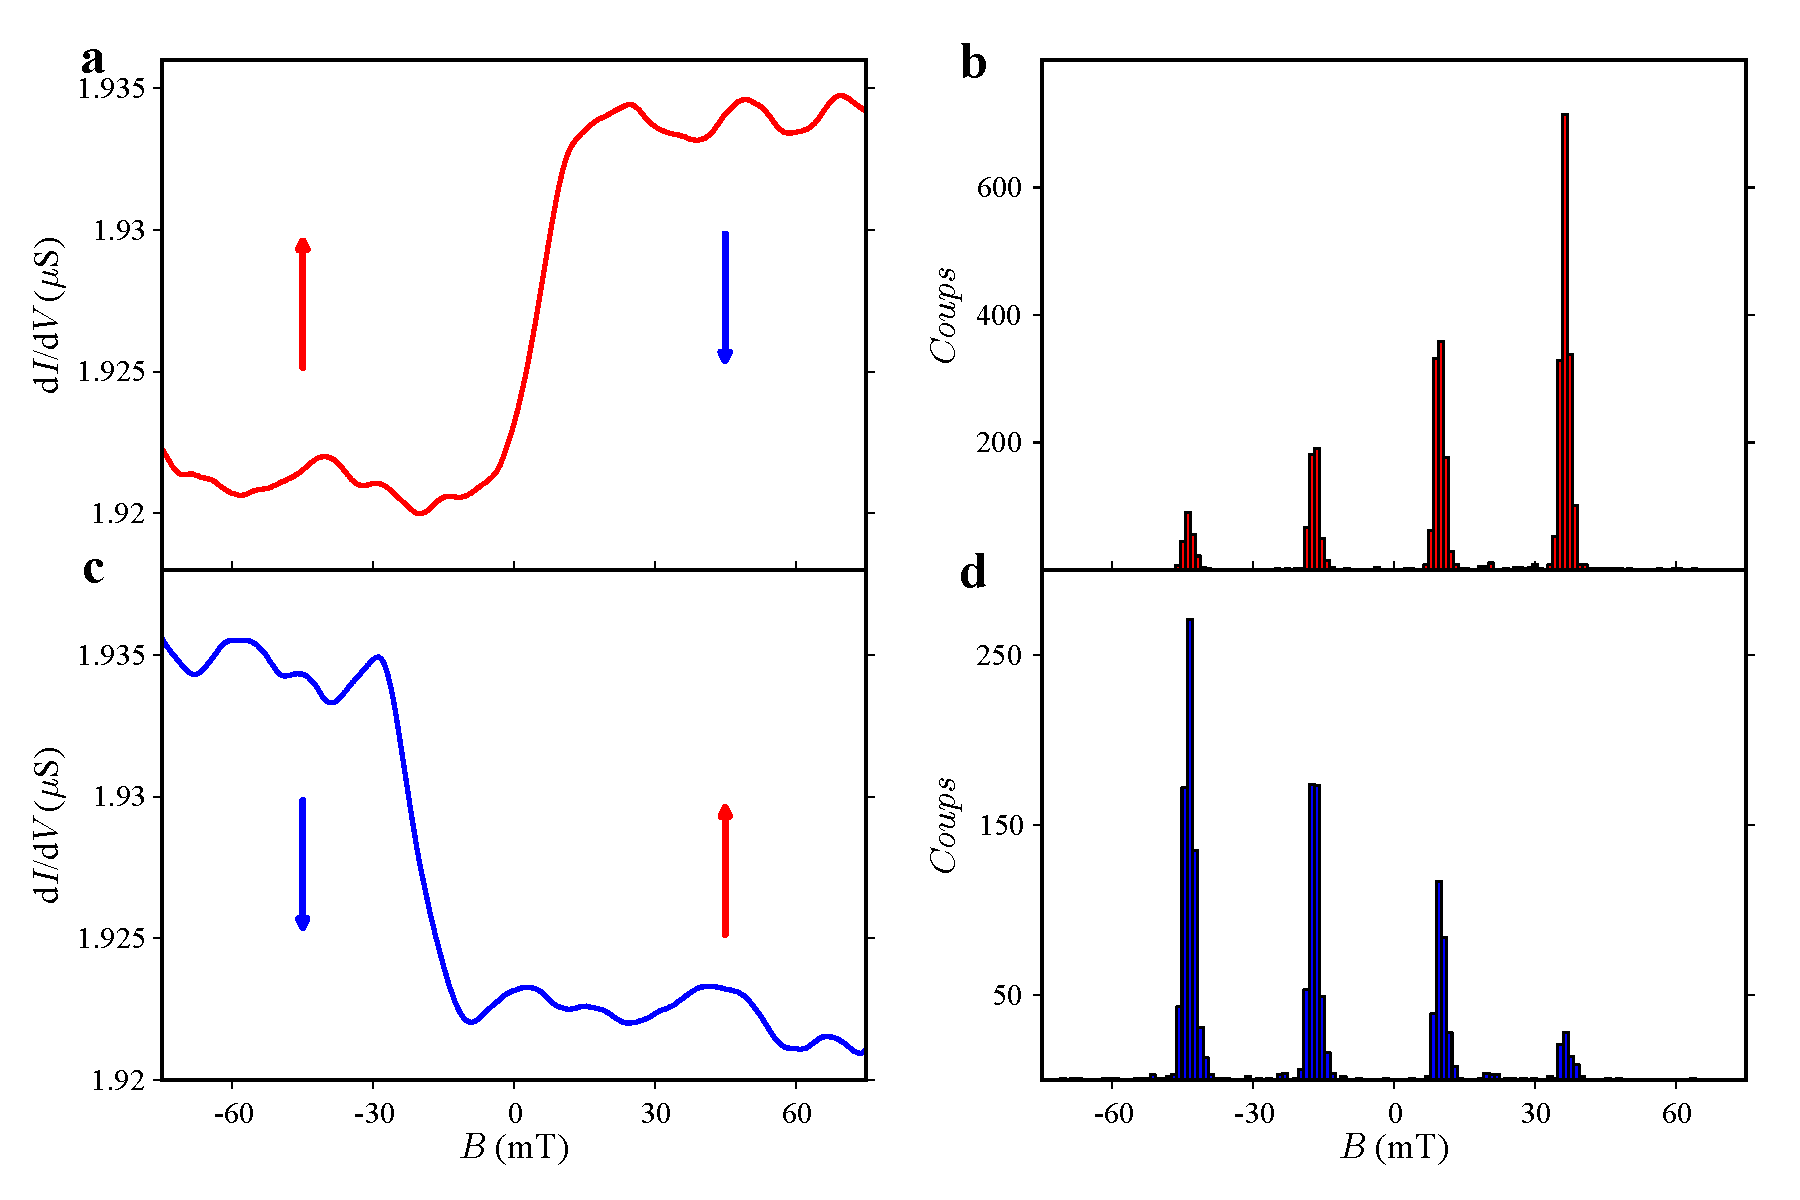
\includegraphics[scale=0.5]{Resultats/Chap1/Figure4/figure4.pdf} 
\caption{}
\label{analyse_signe_saut}
\end{figure}

On peut donc affirmer de façon certaine que la variation en conductance $\Delta G$ est directement lié au retournement de l'aimantation et que son signe nous renseigne sur le sens de la transition.

\subsection{Choix du point de fonctionnement}
Nous avons vu dans la partie théorique consacrée au transport que la zone où la variation de conductance était la plus sensible au potentiel chimique se situe au niveau des points de dégénérescence. C'est dans cette zone que l'on va logiquement se placer. Dans un système idéal, on a $\frac{\partial G}{\partial \mu}_{\text{droite}} = -\frac{\partial G}{\partial \mu}_{\text{gauche}} $. Cela notamment était mis en évidence par [JP,SHUBA] dans le cadre de nanoparticule magnétiques couplé par effet magnéto-Coulomb à un nanotube.

\begin{figure}
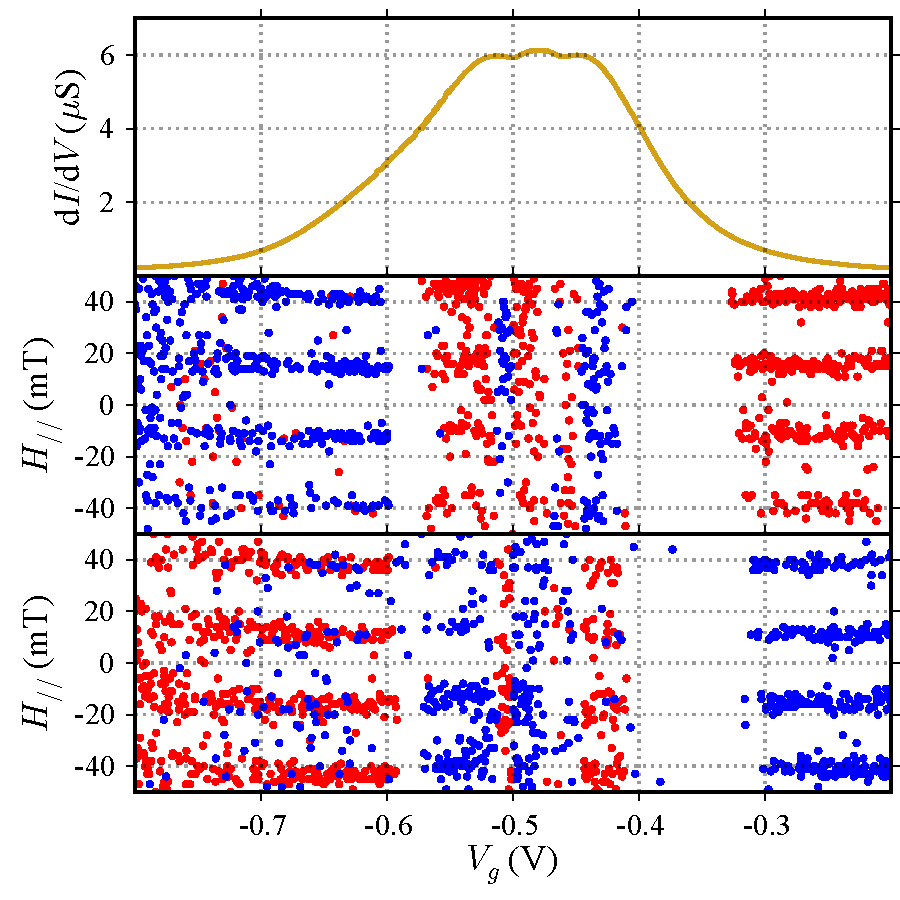
\includegraphics[scale=0.5]{Resultats/Chap1/Figure6/figure6.pdf} 
\caption{}
\label{point_fonctio}
\end{figure}

Dans notre système, cette propriétés n'est pas respecté et le résultat obtenu est plus complexe. La Fig?? montre la signe du changement de conductance correspondant à un retournement, en fonction de la tension de grille $V_g$. On observe trois type de zones : les zones où le signal est trop faible pour être détecté; des zones où le bruit généré par les phénomène de transport masque le signal magnétique.; enfin des zones où le signal magnétique est clair et les résonances clairement visibles. Dans ces dernières, on observe des transitions d'un signe à l'autre similaire à un changement de signe de $\frac{\partial G}{\partial \mu}$. Notre système est en cela relativement éloigné du système idéal que nous avons utilisé jusqu'à maintenant. Et si ce dernier permet de comprendre facilement le couplage magnétisme-transport dans les zone ou $\frac{\partial G}{\partial \mu} = cst$, l'origine des zones de transitions ne nous apparaît toujours pas claire.

\section{Procédure d'alignement}
L'une des caractéristiques principales d'un aimant moléculaire est de posséder un axe facile, c'est à dire, une axe le long duquel le moment magnétique "préfère" s'aligner. C'est suivant cet axe que le champ magnétique nécessaire au retournement de l'aimantation est le plus faible. Pour cette raison, il est indispensable de l'identifier de façon à minimiser le champ magnétique à appliquer à l'échantillon. Dans le cas d'un mauvais alignement, seule la projection suivant l'axe facile du champ magnétique contribue au retournement. Dans le cas extrême où le champ appliqué serait perpendiculaire à cette axe, aucun retournement ne pourrait être observé.

Expérimentalement, le présence d'un retournement peut se mesurer à travers l'apparition d'un hystérésis dans la mesure de conductance. Celui-ci apparait lorsque l'on balaie le champ magnétique des valeurs négatives aux valeurs positives et inversement, tout en mesurant le conductance du système. La Fig.?? mets en évidence cet hystérésis. Une lecture plus claire peut être obtenue en soustrayant l'aller au retour comme le montre la Fig.??. En effectuant cette mesure pour différent angle de champ magnétique, on obtient la mesure de la Fig.???. Celle-ci met clairement en évidence un "axe facile" le long duquel le retournement se fait à faible champ, et un axe difficile le long duquel le champ n'est pas suffisant pour observé de retournement.

\begin{figure}
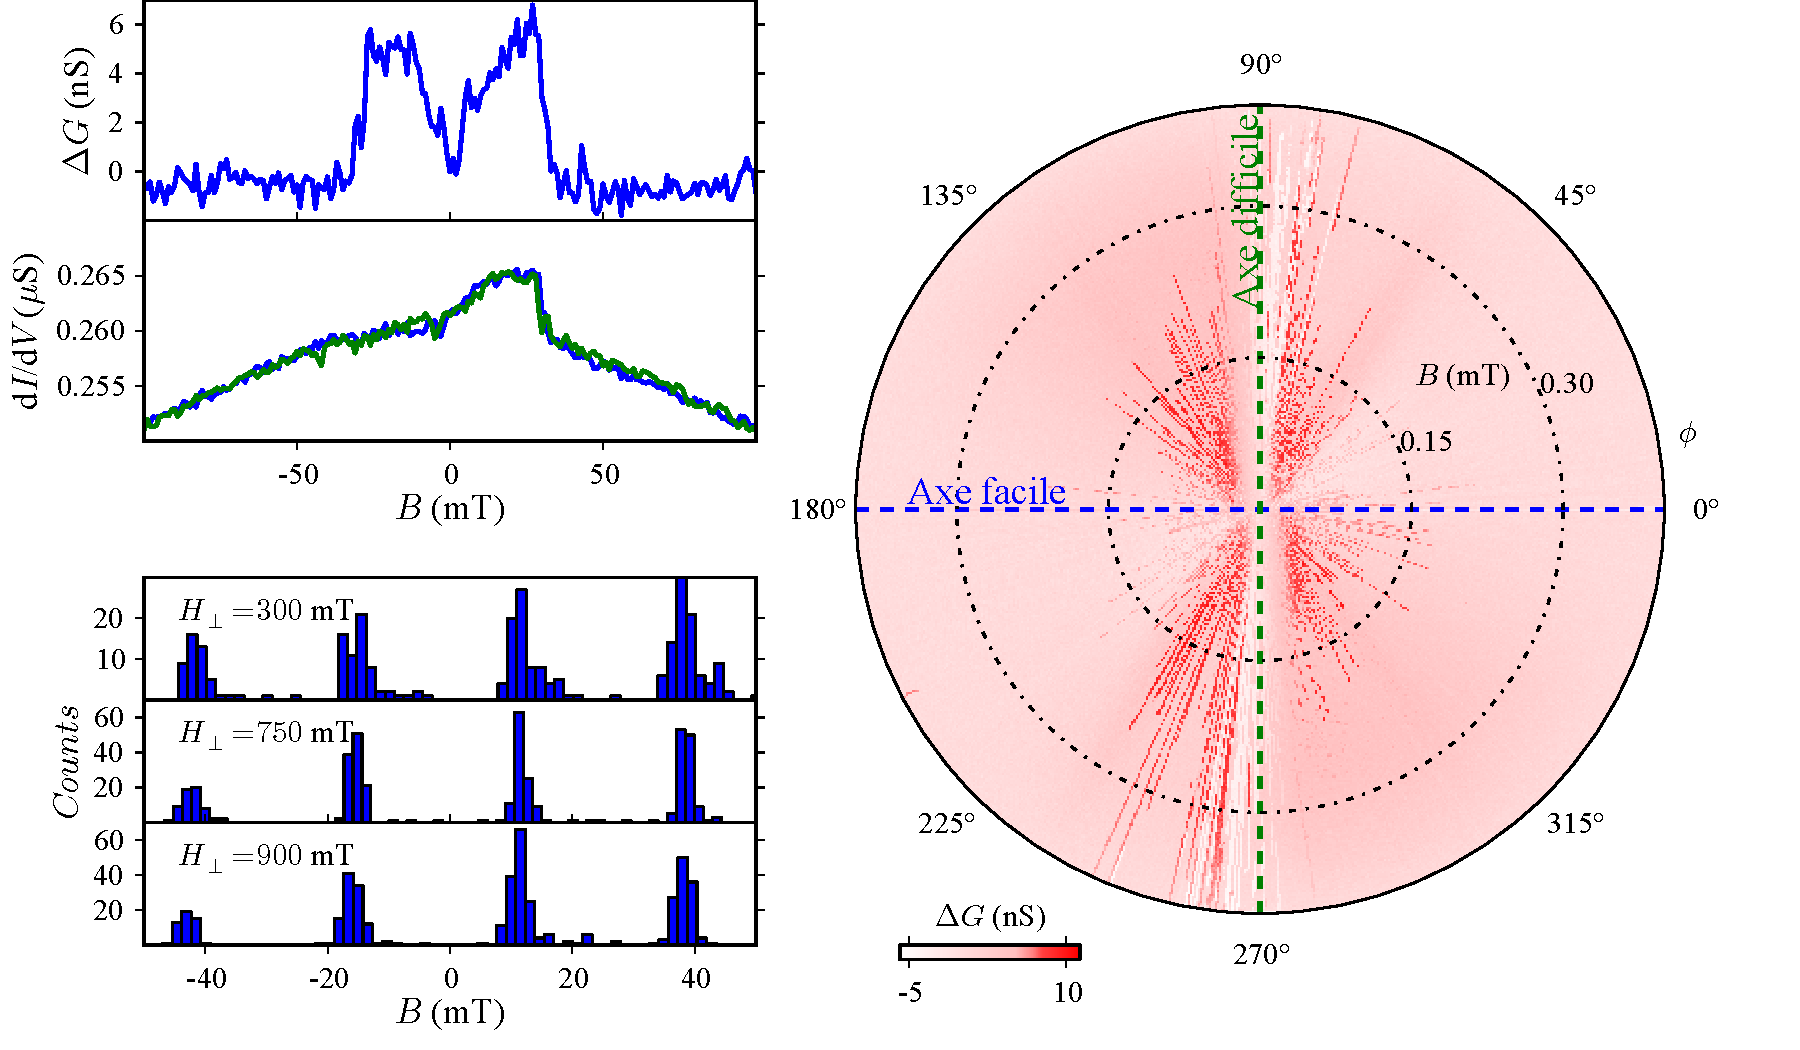
\includegraphics[scale=0.5]{Resultats/Chap1/Figure5/figure5.pdf} 
\caption{}
\label{alignement}
\end{figure}

Cependant, il faut garder à l'esprit que l'"axe facile" identifié sur cette figure n'est en fai que la projection de celui-ci dans le plan défini par la mesure. Il nous faut effectuer une deuxième mesure dans un plan différent pour obtenir un deuxième axe difficle et ainsi pourvoir définir le plan difficile. Sachant que l'axe facile est orthonormal à celui-ci, un produit vectoriel de deux vecteur appartenant au plan difficile nous donne l'axe facile. Expérimentalement, l'angle $\theta$ permetant d'obtenir la Fig.?? est défini à l'aide de deux bobines. L'angle $\phi$ nous permettant de faire la mesure dans deux plans différents est, quant à lui, obtenu par rotation de la dilution le long de l'axe d'une des bobines.


Une méthode permet de vérifier si cet alignement est correct.  Elle consiste à mesurer la positions des résonances à faible champ en fonction d'un champ que l'on applique dans le plan difficile, et que l'on appellera dans la suite champ transverse. Si alignement est correct, la projection d'un tel champ sur l'axe facile est nulle. La position des résonances de devrait donc pas varier. La Fig.??? présente la position de ces résonances pour deux champ transverses. Cette mesure confirme le bon alignement de nos axes magnétiques avec l'axe facile de la molécule.